%%%%%%%%%%%%%%%%%%%%%%%%%%%%%%%%%%%%%%%%%%%%%%%%%%%%%%%%%%%%%%%%%%%%%%
% Problem statement
\begin{statement}[
  problempoints=100,
  timelimit=2 sekunde,
  memorylimit=512 MiB,
]{Bolivija}

Bolivija, predivna južnoamerička država s bogatom kulturom i povijesti, 
prepuna prirodnih ljepota, uključujući dio Amazonske prašume te planinski lanac Ande. 
Bitnije za naše natjecatelje, to je mjesto održavanja sljedeće Međunarodne informatičke 
olimpijade! 

U sklopu promocije natjecanja, organizatori su dobili zadatak 
fotografirati planinski lanac te sastaviti album od najzapanjujućih slika.
Planinski lanac predstavljamo nizom $v$ od $N$ nenegativnih cijelih brojeva koji 
predstavljaju redom visine planina u planinskom lancu. 
Pri tome, $N$ je neparan i središnja planina (na poziciji $\frac{N+1}{2}$) je upravo ona najviša, 
na čijem je samom vrhu ugasli vulkan Nevado Sajama. 

Organizatori imaju vrlo specifične uvjete za prikupljanje fotografija. 
Prvo, biraju dva nenegativna cijela broja $A$ i $B$ tako da je $A < B$ te da je $B$ manji ili 
jednak visini najvišeg vrha, Nevado Sajame. 
Zatim, namještaju kadar fotografije tako da širinom obuhvaća svih $N$ planina, no tako 
da fotografija obuhvaća samo raspon visina između $A$ i $B$. 
Dodatno, organizatori su zadovoljni fotografijom samo ukoliko je ona simetrična s 
obzirom na os simetrije koja prolazi središnjom planinom. 

\begin{figure}[!h]
      \centering
      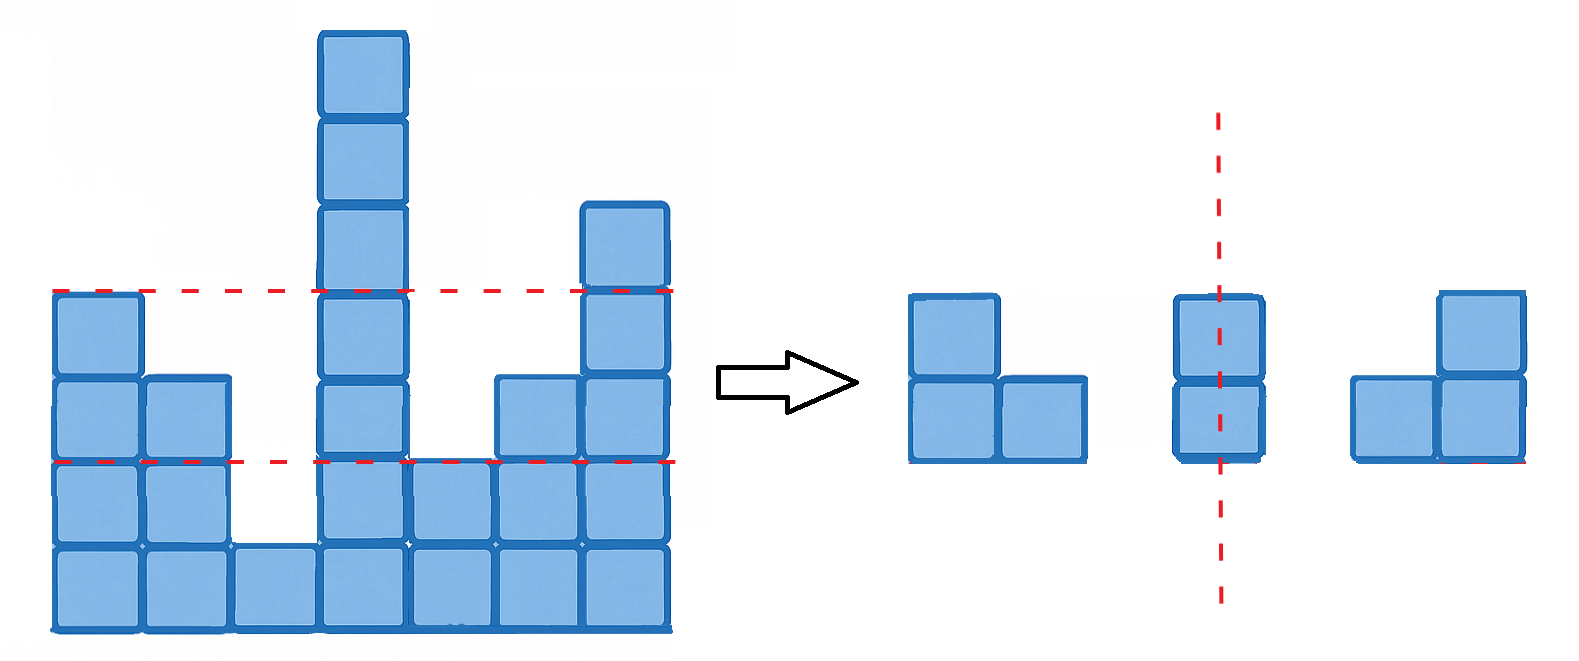
\includegraphics[width=\linewidth]{pic/planine.png}
      \caption*{Slika: Primjer valjanog izbora fotografije koji odgovara drugom probnom primjeru}
\end{figure}

Organizatore sada zanima koliko različitih fotografija mogu prikupiti, odnosno 
koliko postoji parova brojeva $A$ i $B$ koji zadovoljavaju željene uvjete. 
Razmišljajući predugo o odgovoru, burna tektonska aktivnost dovela je do promjene 
visina nekih planina. Ukupno se dogodilo $Q$ promjena visina, a vaš je zadatak 
pomoći organizatorima odrediti traženi broj fotografija nakon svake od promjena. 
Pri tome, nijedna od promjena nije utjecala na visinu središnje planine i ona je 
u svakom trenutku bila najviša planina. 

%%%%%%%%%%%%%%%%%%%%%%%%%%%%%%%%%%%%%%%%%%%%%%%%%%%%%%%%%%%%%%%%%%%%%%
% Input
\subsection*{Ulazni podaci}

U prvom su retku prirodni brojevi $N$ i $Q$, redom broj planina i broj promjena.

U drugom je retku niz $v$ od $N$ nenegativnih cijelih brojeva, redom visine planina u planinskom lancu. 
Garantirano je da je $N$ neparan te da je središnja planina upravo ona najviša. 

U $i$-tom od sljedećih $Q$ redaka su prirodan i nenegativan cijeli broj $x_i$ i $h_i$ ($1 \leq x_i \leq N$), 
koji označavaju da je došlo do promjene visine planine na poziciji $x_i$ koja poprima 
novu visinu $h_i$. Garantirano je da $x_i \ne \frac{N+1}{2}$ te da je nova visina manja 
ili jednaka visini središnje planine. 

%%%%%%%%%%%%%%%%%%%%%%%%%%%%%%%%%%%%%%%%%%%%%%%%%%%%%%%%%%%%%%%%%%%%%%
% Output
\subsection*{Izlazni podaci}

Ispišite $Q + 1$ redaka. U $i$-tom retku ispišite traženi mogući broj fotografija 
nakon $i - 1$ tektonskih promjena. 

%%%%%%%%%%%%%%%%%%%%%%%%%%%%%%%%%%%%%%%%%%%%%%%%%%%%%%%%%%%%%%%%%%%%%%
% Scoring
\subsection*{Bodovanje}

U svim podzadacima vrijedi $3 \leq N \leq 200~000$ i $0 \leq Q \leq 200~000$. 

Za sve $i = 1, \dots, N$ vrijedi da je $v_i \leq 654~200$ 
(visina vrha Nevado Sajama u centimetrima). 

{\renewcommand{\arraystretch}{1.4}
  \setlength{\tabcolsep}{6pt}
  \begin{tabular}{ccl}
   Podzadatak & Broj bodova & Ograničenja \\ \midrule
    1 & 9 & $Q = 0, N \leq 300,$ te $v_i \leq 300$ za sve $i = 1, \dots, N$ \\
    2 & 23 & $Q = 0$ \\
    3 & 31 & Svaka promjena mijenja visinu planine najviše za $1$.  \\
    4 & 37 & Nema dodatnih ograničenja. \\
\end{tabular}}

%%%%%%%%%%%%%%%%%%%%%%%%%%%%%%%%%%%%%%%%%%%%%%%%%%%%%%%%%%%%%%%%%%%%%%
% Examples
\subsection*{Probni primjeri}
\begin{tabularx}{\textwidth}{X'X'X}
\sampleinputs{test/bolivija.dummy.in.1}{test/bolivija.dummy.out.1} &
\sampleinputs{test/bolivija.dummy.in.2}{test/bolivija.dummy.out.2} &
\sampleinputs{test/bolivija.dummy.in.3}{test/bolivija.dummy.out.3}
\end{tabularx}

\textbf{Pojašnjenje drugog probnog primjera:}

Mogući izbori za $A$ i $B$ su: 
$(0, 1), (2, 3), (2, 4), (3, 4), (5, 6), (5, 7), (6, 7)$. 
Ukupno ih je sedam. 

Slika u tekstu odgovara odabiru $A = 2$ i $B = 4$.

%%%%%%%%%%%%%%%%%%%%%%%%%%%%%%%%%%%%%%%%%%%%%%%%%%%%%%%%%%%%%%%%%%%%%%
% We're done
\end{statement}

%%% Local Variables:
%%% mode: latex
%%% mode: flyspell
%%% ispell-local-dictionary: "croatian"
%%% TeX-master: "../hio.tex"
%%% End:
